\def\mySecNum{3.3}
\mySection{\mySecNum~Spreads and collars}
%-------------- start slide -------------------------------%{{{ 1
\begin{frame}[fragile]
\begin{center}
	It is always possible                             \\
	\bigskip
	to                                                \\
	\bigskip
	\textcolor{magenta}{lower the cost of a position} \\
	\bigskip
	by                                                \\
	\bigskip
	\textcolor{cyan}{reducing its payoff!}
\end{center}
\end{frame}
%-------------- end slide -------------------------------%}}}
%-------------- start slide -------------------------------%{{{ 1
\begin{frame}[fragile,t]
	\begin{center}
		By combining two or more options, we find many well-known strategies.

	\bigskip

	\begin{center}
		\begin{tikzpicture}[scale=1, transform shape]
			\tikzset{>=latex}
			\draw[thick,->] (-0.3,0.3) -- (7,0.3);
			\draw[thick,->] (0,0) -- (0,6.5);
			\node (LC) at (2,2) {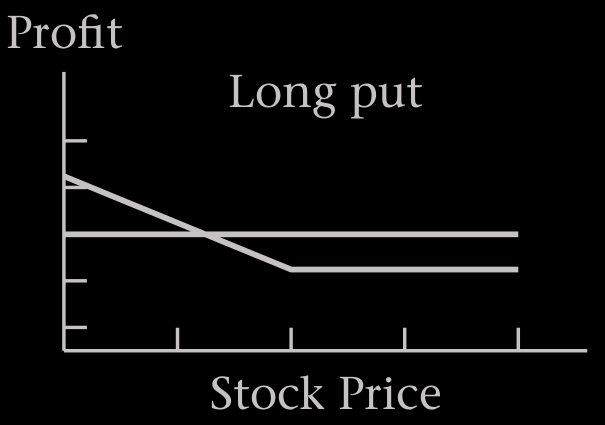
\includegraphics[scale=0.15]{figs/Long-put.png}};
			\node (LC) at (2,5) {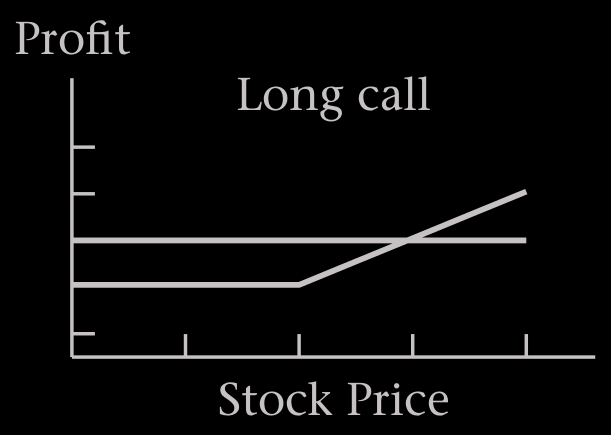
\includegraphics[scale=0.15]{figs/Long-call.png}};
			\node (LC) at (5,2) {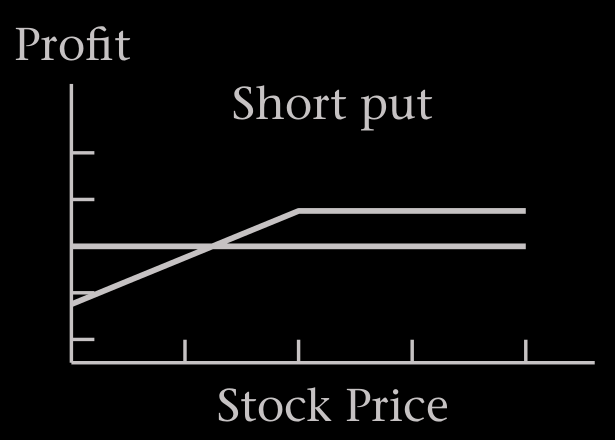
\includegraphics[scale=0.15]{figs/Short-put.png}};
			\node (LC) at (5,5) {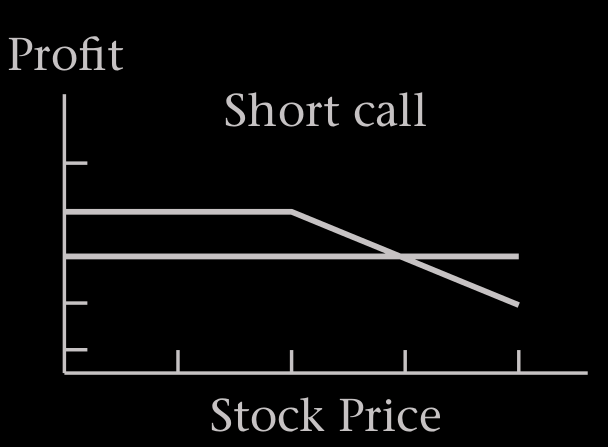
\includegraphics[scale=0.15]{figs/Short-call.png}};
			\draw[thick] (2,0.5) -- ++ (0,-0.5) node [below] {Long};
			\draw[thick] (5,0.5) -- ++ (0,-0.5) node [below] {Short};
			\draw[thick] (0.2,5) -- ++ (-0.5,0) node [left] {Call};
			\draw[thick] (0.2,2) -- ++ (-0.5,0) node [left] {Put};
		\end{tikzpicture}
	\end{center}
	\end{center}
\end{frame}
%-------------- end slide -------------------------------%}}}
%-------------- start slide -------------------------------%{{{ 1
\begin{frame}[fragile]
	\begin{center}
	\begin{center}
		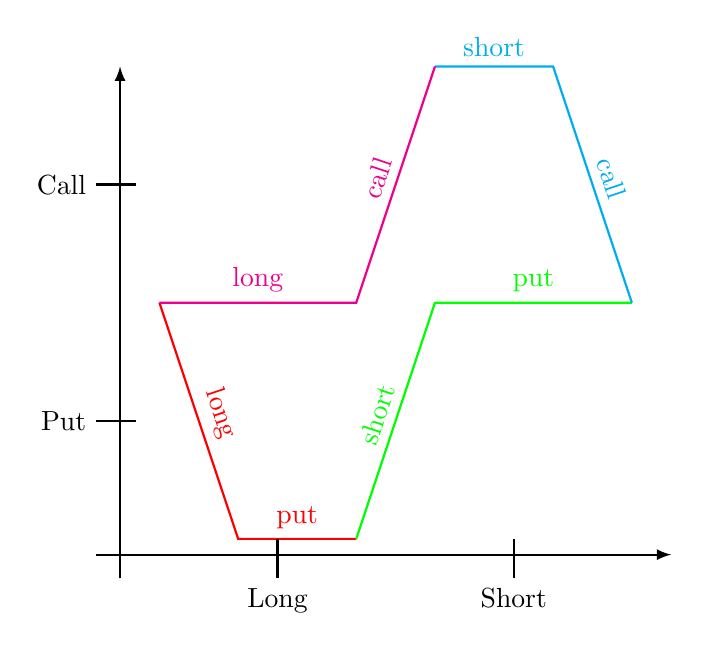
\begin{tikzpicture}[scale=1, transform shape]
			\tikzset{>=latex}
			\draw[thick,->] (-0.3,0.3) -- (7,0.3);
			\draw[thick,->] (0,0) -- (0,6.5);
			% \node (LC) at (2,2) {\includegraphics[scale=0.15]{figs/Long-put.png}};
			% \node (LC) at (2,5) {\includegraphics[scale=0.15]{figs/Long-call.png}};
			% \node (LC) at (5,2) {\includegraphics[scale=0.15]{figs/Short-put.png}};
			% \node (LC) at (5,5) {\includegraphics[scale=0.15]{figs/Short-call.png}};
			\draw[thick,red] (0.5,3.5) -- (1.5,0.5)  node [midway,above, sloped] {long} -- (3,0.5) node [midway,above, sloped, red] {put};
			\draw[thick,green] (3,0.5) -- (4,3.5) node [midway, above, sloped] {short} -- (6.5,3.5) node [midway, above, sloped] {put};
			\draw[thick,cyan] (6.5,3.5) -- (5.5,6.5) node [midway, above, sloped] {call} -- (4,6.5) node [midway, above, sloped] {short};
			\draw[thick,magenta] (4,6.5) -- (3,3.5) node [midway, above, sloped] {call} -- (0.5,3.5) node [midway, above, sloped] {long};

			\draw[thick] (2,0.5) -- ++ (0,-0.5) node [below] {Long};
			\draw[thick] (5,0.5) -- ++ (0,-0.5) node [below] {Short};
			\draw[thick] (0.2,5) -- ++ (-0.5,0) node [left] {Call};
			\draw[thick] (0.2,2) -- ++ (-0.5,0) node [left] {Put};
		\end{tikzpicture}
	\end{center}
	\end{center}
\end{frame}
%-------------- end slide -------------------------------%}}}
%-------------- start slide -------------------------------%{{{ 1
\begin{frame}[fragile,t]

	An \textcolor{magenta}{option spread} is a position consisting of only calls or only puts, in
	which some options are purchased and some written.
	\bigskip

	\begin{itemize}
		\item Bull and bear spreads
			\bigskip
		\item Box spreads
			\bigskip
		\item Ratio spreads
			\bigskip
		\item Collars
	\end{itemize}


\end{frame}
%-------------- end slide -------------------------------%}}}
%-------------- start slide -------------------------------%{{{ 1
\begin{frame}[fragile,t]
	\frametitle{Example for this section}
	\begin{center}
		Black-Scholes option prices \\
		\begin{align*}
			\text{Stock price}                     & = \$40   \\
			\text{Volatility}                      & = 30\%   \\
			\text{Effective annual risk-free rate} & = 8.33\% \\
			\text{Dividend yield} & = \$0 \\
			\text{Expriation days} & = 91~\text{days}
		\end{align*}

		\bigskip
		\renewcommand{\arraystretch}{1.2}
		\begin{tabular}{ccc}
			\hline
			Strike & Call & Put  \\
			\hline
			35     & 6.13 & 0.44 \\
			40     & 2.78 & 1.99 \\
			45     & 0.97 & 5.08 \\
		\end{tabular}
		\end{center}
\end{frame}
%-------------- end slide -------------------------------%}}}
%-------------- start slide -------------------------------%{{{ 1
\begin{frame}[fragile,t]
	\frametitle{Bull and bear spreads}

	\bigskip
	A position in which you buy a call and sell  an otherwise identical call with a higher strike price
	is an example of a \textcolor{magenta}{bull spread}. Bull spreads can also be constructed using
	puts.

	\bigskip
	The opposite of a bull spread is a \textcolor{magenta}{bear spread}.

\end{frame}
%-------------- end slide -------------------------------%}}}
%-------------- start slide -------------------------------%{{{ 1
\begin{frame}[fragile]
	\begin{center}
		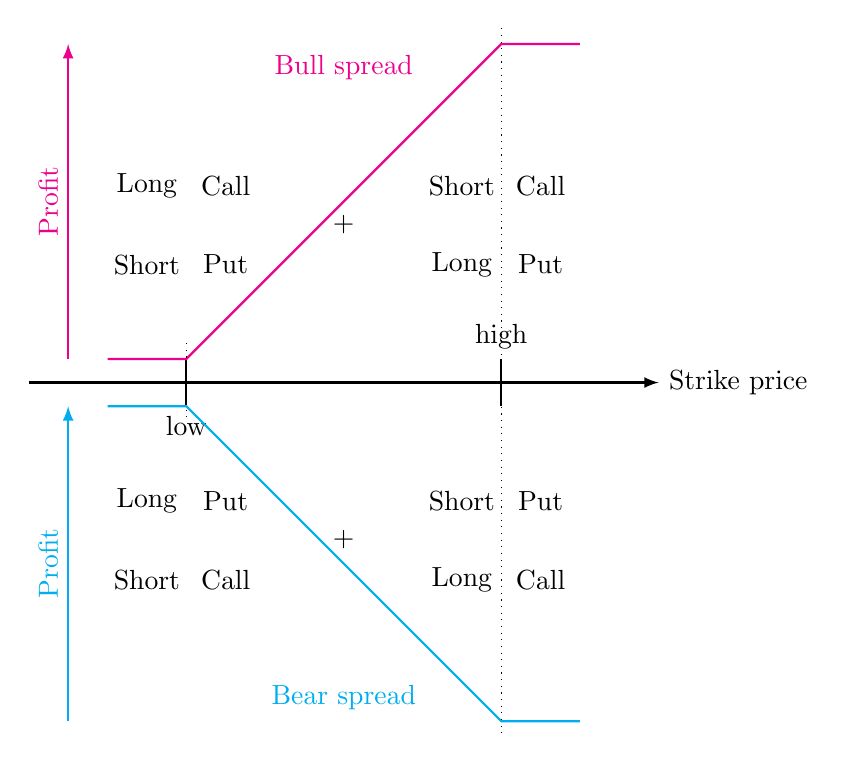
\begin{tikzpicture}[scale=1, transform shape]
			\tikzset{>=latex}
			\draw[->, thick] (-4,0) -- (4,0) node [right] {Strike price};
			\draw[thick] (-2,0.3) -- ++(0,-0.6) node [below] {low};
			\draw[thick] (2,-0.3) -- ++(0,0.6) node [above] {high};
			\pause
			\node at (0,4) {\textcolor{magenta}{Bull spread}};

			\pause
			% \draw (-1.9,2) circle (1.2);
			\node at  (-2.5,2.5) {Long};
			\node at  (-1.5,2.5) {Call};
			\node at  (-2.5,1.5) {Short};
			\node at  (-1.5,1.5) {Put};

			\pause
			% \draw (1,1) rectangle (3,3);
			\node at  (1.5,2.5) {Short};
			\node at  (2.5,2.5) {Call};
			\node at  (1.5,1.5) {Long};
			\node at  (2.5,1.5) {Put};
			\node at (0,2) {$+$};

			\pause
			\node at (0,-4) {\textcolor{cyan}{Bear spread}};

			\pause
			% \draw (-1,-1) rectangle (-3,-3);
			\node at  (-2.5,-1.5) {Long};
			\node at  (-1.5,-1.5) {Put};
			\node at  (-2.5,-2.5) {Short};
			\node at  (-1.5,-2.5) {Call};

			\pause
			% \draw (1.9,-2) circle (1.2);
			\node at  (1.5,-1.5) {Short};
			\node at  (2.5,-1.5) {Put};
			\node at  (1.5,-2.5) {Long};
			\node at  (2.5,-2.5) {Call};

			\node at (0,-2) {$+$};

			\pause
			\draw[magenta, thick] (-3,0.3) -- (-2,0.3) -- (2,4.3) -- (3,4.3);
			\draw[cyan, thick] (-3,-0.3) -- (-2,-0.3) -- (2,-4.3) -- (3,-4.3);
			\draw[dotted] (2,4.5) -- ++ (0,-9);
			\draw[dotted] (-2,0.5) -- ++ (0,-1);
			\draw[thick,->,magenta] (-3.5,0.3) -- ++ (0, 4) node [midway,sloped,above] {Profit};
			\draw[thick,->,cyan] (-3.5,-4.3) -- ++ (0, 4) node [midway,sloped,above] {Profit};
		\end{tikzpicture}
	\end{center}
\end{frame}
%-------------- end slide -------------------------------%}}}
%-------------- start slide -------------------------------%{{{ 1
\begin{frame}[fragile,t]
	\begin{myexample}
		Draw profit diagram for a 40-45	bull spread, namely, buying a 40-strike call and selling
		a 45-strike call.
	\end{myexample}
	\pause
	\begin{mysol}\phantom{a}\\
		\begin{center}
			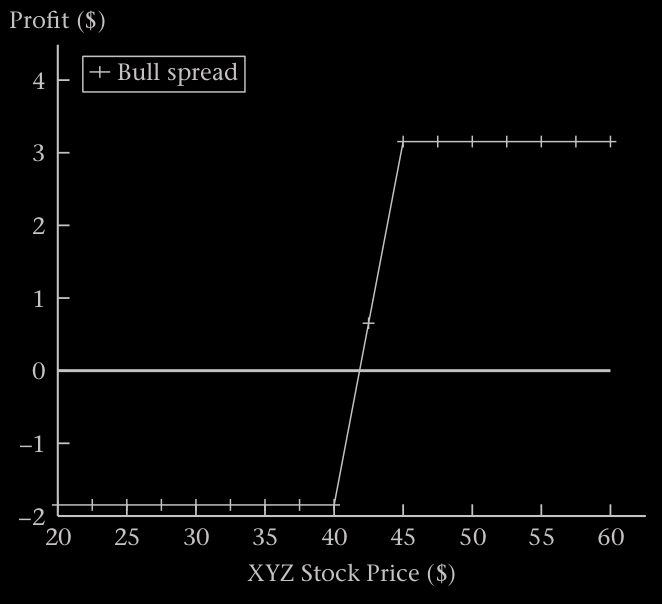
\includegraphics[scale=0.2]{figs/Figure-3-7.png}
		\end{center}

		We only need to determine the two levels.
	\end{mysol}
\end{frame}
%-------------- end slide -------------------------------%}}}
%-------------- start slide -------------------------------%{{{ 1
\begin{frame}[fragile,t]
	\begin{mysol}[(Continued)]\\
		\bigskip

		(a)	 Suppose that the index price is \$ 30 at the expiration:
		\begin{align*}
			\left(\$ 2.78 - \$ 0.97 \right) \times (1+0.0833)^{1/4} = \textcolor{magenta}{\$ 1.85}.
		\end{align*}
		\bigskip \pause

		(b) Suppose that the index price is \$50 at the expiration:
		\begin{align*}
			(\$50 - \$40) - (\$ 40 - \$ 45) - \textcolor{magenta}{\$ 1.85} = \$ 3.15.
		\end{align*}
		\myEnd
	\end{mysol}
\end{frame}
%-------------- end slide -------------------------------%}}}
%-------------- start slide -------------------------------%{{{ 1
\begin{frame}[fragile,t]
	\frametitle{Box spreads}

	A \textcolor{magenta}{\bf box spread} is accomplished by using options to create
	\textcolor{magenta}{a synthetic long forward} at one price and \textcolor{cyan}{a synthetic short
	forward} at a different price.
	\bigskip

	This strategy guarantees a cash flow in the future.
	\bigskip

	Hence, it is an option spread that is purely a means of borrowing or lending money. It is costly
	but has no stock price risk.
\end{frame}
%-------------- end slide -------------------------------%}}}
%-------------- start slide -------------------------------%{{{ 1
\begin{frame}[fragile,t]
\begin{myexample}
	Suppose we simultaneously enter into the following two transactions:
	\begin{enumerate}
		\item Buy a 40-strike call and sell a 40-strike put.
		\item Sell a 45-strike call and buy a 45-strike put.
	\end{enumerate}
	\pause
	Explain why there is no free lunch. Draw the profit diagram.
\end{myexample}
\bigskip
\pause
\begin{mysol}
	The profit is
	\begin{align*}
		5 + \underbrace{(1.99-2.78)\times (1.0833)^{1/4}}_{\text{Synthetic long forward}}
		+ \underbrace{(0.97-5.08)\times (1.0833)^{1/4}}_{\text{Synthetic short forward}}
		= \$ 0.0099851.
	\end{align*}
  %
	% 5 + (1.99-2.78)*(1.0833)**0.25 +(0.97-5.08)*(1.0833)**0.25
  %
	\myEnd
\end{mysol}
\end{frame}
%-------------- end slide -------------------------------%}}}
%-------------- start slide -------------------------------%{{{ 1
\begin{frame}[fragile]
\begin{center}
	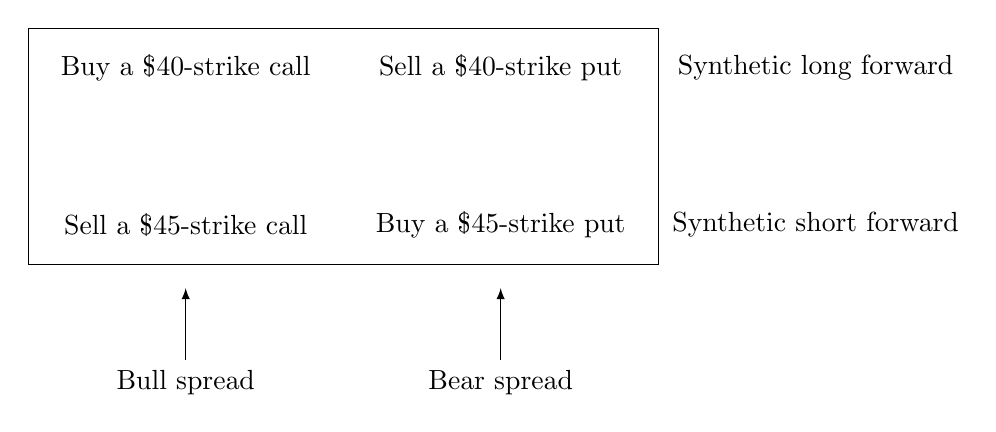
\begin{tikzpicture}[scale=1, transform shape]
		\tikzset{>=latex}
		\node[] (a) at (-2,+1) {Buy  a \$40-strike call}; \node[] (a) at (+2,+1) {Sell a \$40-strike put};
		\node[] (a) at (-2,-1) {Sell a \$45-strike call}; \node[] (a) at (+2,-1) {Buy  a \$45-strike put};
		\node[] (b) at (-2,-3) {Bull spread}; \draw [->] (b) -- ++(0,1.2);
		\node[] (b) at (+2,-3) {Bear spread}; \draw [->] (b) -- ++(0,1.2);
		\node[] (c) at (6,1) {Synthetic long forward};
		\node[] (c) at (+6,-1) {Synthetic short forward};
		\draw (-4,-1.5) rectangle (4,1.5);
	\end{tikzpicture}
\end{center}
\end{frame}
%-------------- end slide -------------------------------%}}}
%-------------- start slide -------------------------------%{{{ 1
\begin{frame}[fragile,t]
	\frametitle{Ratio spreads}

	A \textcolor{magenta}{\bf ratio spread} is constructed by buying m options at one strike and
	selling n options at a different strike, with all options having the same type (call or put), same
	time to maturity, and same underlying asset.
	\bigskip

	\begin{center}
		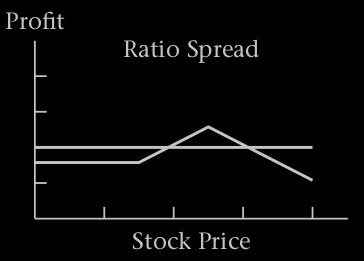
\includegraphics[scale=0.3]{figs/Profit_Ratio_Spread.png}
	\end{center}

\end{frame}
%-------------- end slide -------------------------------%}}}
%-------------- start slide -------------------------------%{{{ 1
\begin{frame}[fragile,t]
	\begin{myexample}[(Problem 3.15)]
	Compute profit diagrams for the following ratio spreads:
	\begin{itemize}
		\item[a] Buy 950-strike call, sell two 1050-strike calls.
		\item[b] Buy two 950-strike calls, sell three 1050-strike calls.
		\item[c] Consider buying n 950-strike calls and selling m 1050-strike calls so that the premium of the position is zero. Considering your analysis in (a) and (b), what can you say about n/m? What exact ratio gives you a zero premium?
	\end{itemize}
	\begin{center}
\renewcommand{\arraystretch}{1.2}
		\begin{tabular}{|c|c|c|}
		\hline
		Strike & Call      & Put      \\ \hline
		\$950  & \$120.405 & \$51.777 \\
		1000   & 93.809    & 74.201   \\
		1020   & 84.470    & 84.470   \\
		1050   & 71.802    & 101.214  \\
		1107   & 51.873    & 137.167  \\ \hline
		\end{tabular}
	\end{center}
	\end{myexample}
	\pause
	\begin{mysol}
		\textcolor{gray}{...}	\myEnd
	\end{mysol}
\end{frame}
%-------------- end slide -------------------------------%}}}
%-------------- start slide -------------------------------%{{{ 1
\begin{frame}[fragile,t]
	\frametitle{Collars}

	A \textcolor{magenta}{\bf collar} is the purchase of a put option and the sale of a call option with
	a higher strike price, with both options having the same underlying asset and having the same
	expiration date.

	\bigskip

	If the position is reversed, i.e., sale of a put and purchase of a call, the collar is written.

	\bigskip

	The \textcolor{magenta}{\bf collar width} is the difference between the call and put strikes.
\end{frame}
%-------------- end slide -------------------------------%}}}
%-------------- start slide -------------------------------%{{{ 1
\begin{frame}[fragile,t]
\begin{myexample}
 	Draw the profit diagram for a purchased collar:
	\begin{align*}
		\text{selling a 45-strike call} + \text{buying a 40-strike put}.
	\end{align*}
\end{myexample}
\pause
\bigskip
\begin{mysol}
	One can easily draw the profit graph. We only need to determine the level when the curve is flat. Hence, 
	suppose the price is \$43. Then the profit is
	\begin{align*}
		(0.97-1.99) \times (1.083)^{1/4} = -\$1.0405.
	\end{align*}
	\bigskip

	\begin{center}
		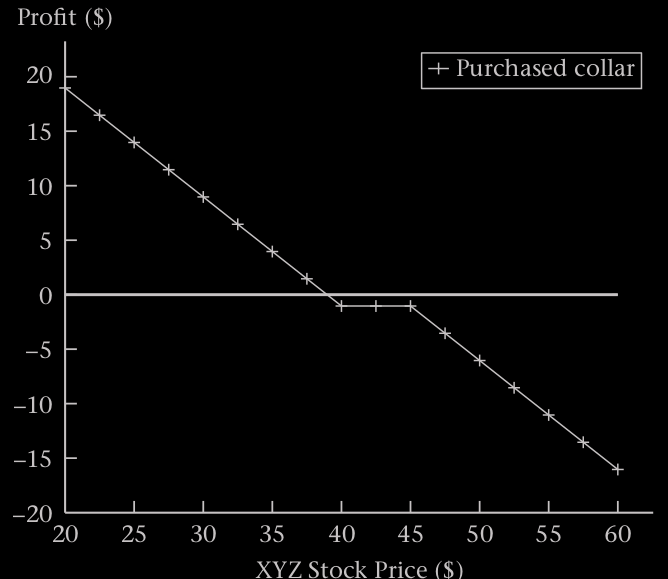
\includegraphics[scale=0.2]{figs/Figure-3-8.png}
	\end{center}
	\myEnd
\end{mysol}
\end{frame}
%-------------- end slide -------------------------------%}}}
%-------------- start slide -------------------------------%{{{ 1
\begin{frame}[fragile,t]
It is possible to find strike prices for the put and call such that the two premiums exactly offset one another. This
position is called a \textcolor{magenta}{\bf zero-cost collar}.
\end{frame}
%-------------- end slide -------------------------------%}}}
%-------------- start slide -------------------------------%{{{ 1
\begin{frame}[fragile,t]
	\begin{myexample}
		Consider XYZ:
		\begin{center}
			\renewcommand{\arraystretch}{1.2}
			\begin{tabular}{ccc}
				\hline
				Strike                     & Call                      & Put                      \\
				\hline
				35                         & 6.13                      & 0.44                     \\
				40                         & 2.78                      & \textcolor{cyan}{1.99}   \\
				\textcolor{magenta}{41.72} & \textcolor{magenta}{1.99} & \textcolor{magenta}{---} \\
				45                         & 0.97                      & 5.08                     \\
			\end{tabular}
		\end{center}
		where we need to use \textcolor{red}{Black-Scholes formula} to find out the strike price, which is \textcolor{magenta}{41.72},
		when the put premium is \textcolor{magenta}{\$1.99}.
		This gives a zero-cost collar.
		% \begin{align*}
		% 	\text{buying XYZ at \$40} + \text{buying a 40-strike put} + \text{selling a 41.72-strike call}
		% \end{align*}
		% Draw the profit diagram.
	\end{myexample}
	% \pause
	% \bigskip
	% \begin{mysol}
	% 	\textcolor{gray}{Check book p. 77.} \myEnd
	% \end{mysol}
\end{frame}
%-------------- end slide -------------------------------%}}}
